\documentclass[linenumbers]{aastex63}
\usepackage{tabularx}
\usepackage{amsmath}

\renewcommand{\thefigure}{S\arabic{figure}}
\renewcommand{\thetable}{S\arabic{table}}

\begin{document}

% Title
\title{Supplementary Information for

Timing and Likelihood of the Origin of Life Derived from Post-Impact Highly Reducing Atmospheres}

% Authors
\author{Nicholas F. Wogan}
\affiliation{Space Science Division, NASA Ames Research Center, Moffett Field, CA 94035}
\affiliation{Virtual Planetary Laboratory, University of Washington, Seattle, WA 98195}

\author{David C. Catling}
\affiliation{Department of Earth and Space Sciences, University of Washington, Seattle, WA 98195}
\affiliation{Virtual Planetary Laboratory, University of Washington, Seattle, WA 98195}

\author{Kevin J. Zahnle}
\affiliation{Space Science Division, NASA Ames Research Center, Moffett Field, CA 94035}
\affiliation{Virtual Planetary Laboratory, University of Washington, Seattle, WA 98195}

\section{Size-frequency distribution sensitivity test} \label{sec:append_sfd}

\begin{figure}
  \centering
  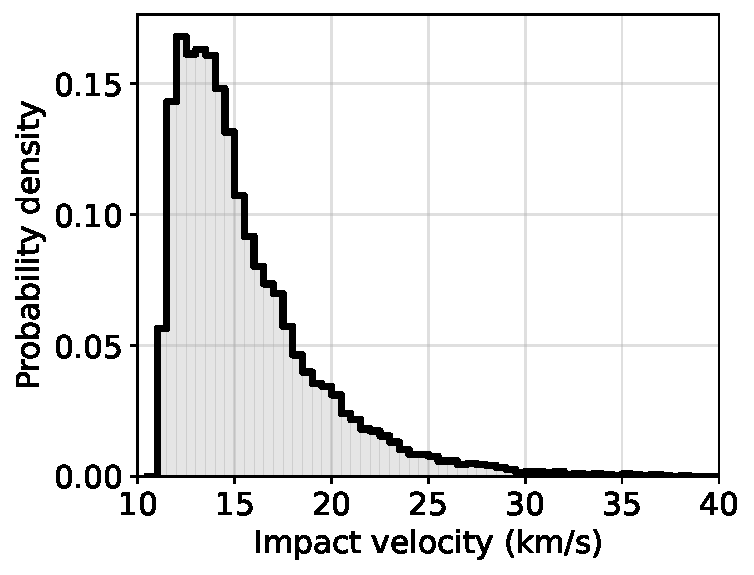
\includegraphics[width=0.4\textwidth]{figures/velocity_distribution.pdf}
  \caption{Our assumed probability distribution for the velocity of impacts derived from modern observations of asteroid close approaches \citep{Park_2023}.}
  \label{fig:velocity_distribution}
\end{figure}

We assume that the size-frequency distribution of objects that struck the early Earth is similar to the main-belt asteroids. A problem with this approach is that the main-belt asteroids only contain objects up to $\sim$ 1000 km diameter, yet the early Earth is expected to have experienced impacts larger than this \citep{Marchi_2014}. Therefore, we must extrapolate the size-frequency distribution above $\sim$ 1000 km to larger objects. Throughout the main text we use the same extrapolation as \citet{Marchi_2014} (the black dashed line in Main Text Figure 4, who extends the size-frequency distribution with a log-log slope of $d (\ln S_0)/d (\ln m) = - 0.415$.

To test the sensitivity of our results to this chosen extrapolation, we re-did our Monte-Carlo analysis using a log-log slope of $d (\ln S_0)/d (\ln m) = - 1$ (the red dashed line in Main Text Figure 4) for impactors bigger than $\sim$ 1000 km diameter. Figures \ref{fig:probabilities_of_impacts_extrapolation_sens} and \ref{fig:timing_extrapolation_sensitivity} show how our results change when adopting this alternative extrapolation. Overall, our results are qualitatively unchanged for the different extrapolation slope ($d (\ln S_0)/d (\ln m)$).

\begin{figure}
  \centering
  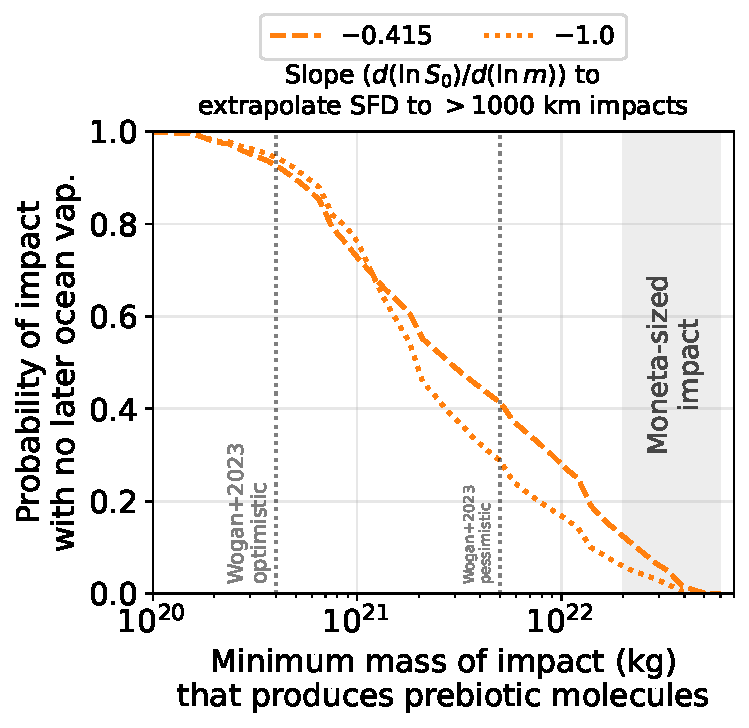
\includegraphics[width=0.5\textwidth]{figures/probabilities_of_impacts_extrapolation_sens.pdf}
  \caption{Similar to Main Text Figure 2, except we consider different extrapolations of the size-frequency distribution (SFD) for impactors larger than 1000 km diameter. The line labeled $d (\ln S_0)/d (\ln m) = - 0.415$ is the black dashed extrapolation in Main Text Figure 4a. The $d (\ln S_0)/d (\ln m) = - 1.0$ case is shown by the red dashed extrapolation in Main Text Figure 4a.}
  \label{fig:probabilities_of_impacts_extrapolation_sens}
\end{figure}

\begin{figure}
  \centering
  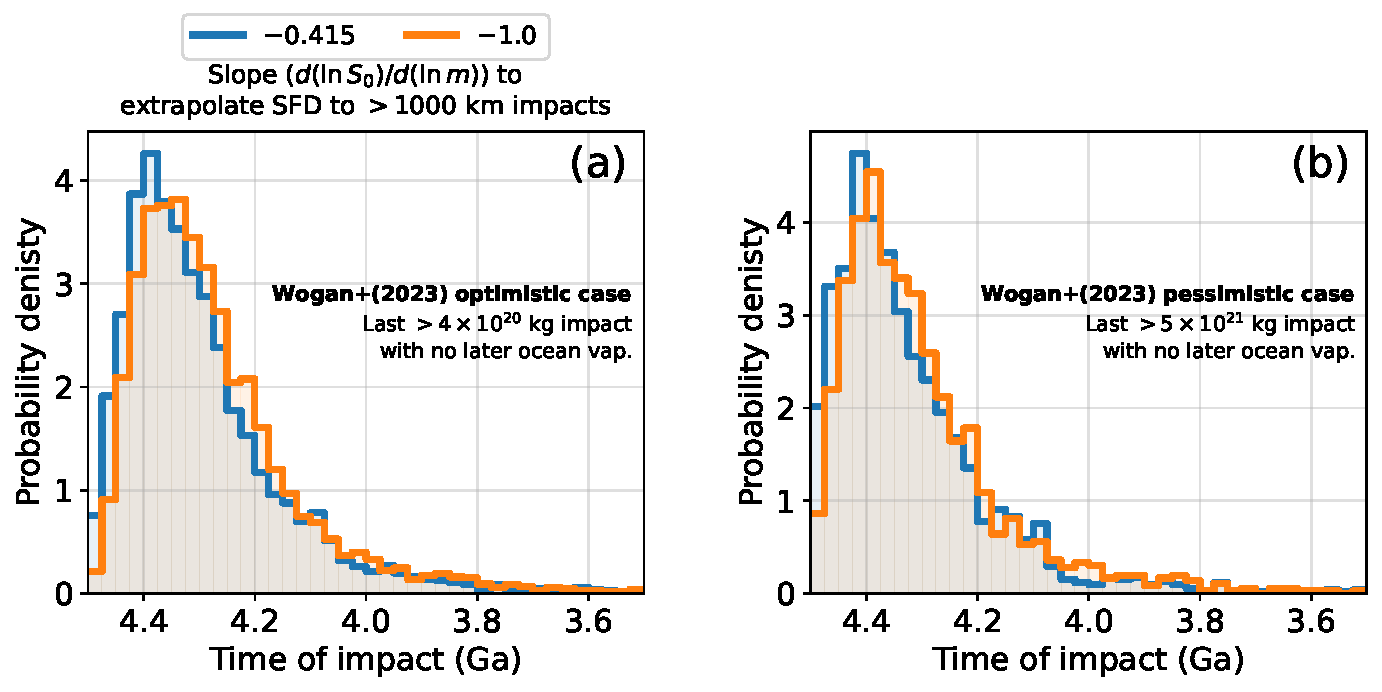
\includegraphics[width=0.85\textwidth]{figures/timing_extrapolation_sensitivity.pdf}
  \caption{Similar to Main Text Figure 3, except we consider different extrapolations of the size-frequency distribution (SFD) for impactors larger than 1000 km diameter. The line labeled $d (\ln S_0)/d (\ln m) = - 0.415$ is the black dashed extrapolation in Main Text Figure 4a. The $d (\ln S_0)/d (\ln m) = - 1.0$ case is shown by the red dashed extrapolation in Main Text Figure 4a.}
  \label{fig:timing_extrapolation_sensitivity}
\end{figure}

\section{Impact energy required for ocean vaporization} \label{sec:append_vap}

Recently, \citet{Citron_2022} performed smoothed-particle hydrodynamics impact simulations over a range of impact angles, masses and velocities to estimate the impact properties that can vaporize an ocean. Figure \ref{fig:energy_for_ocean_vap}a shows their simulation results for the change in the atmosphere's and ocean's internal energy ($\Delta \mathrm{IE}_\mathrm{atmo}$) as a function of impact kinetic energy ($\mathrm{E}_\mathrm{imp}$), along with log-log extrapolations for each impact angle. Figure \ref{fig:energy_for_ocean_vap} gives the same information, but the y-axis is instead the fraction of the impactor's energy that heats the atmosphere and ocean over the course of their simulations. For the most probable incident impact angle of $45^\circ$ about $\sim 10\%$ of the impactors kinetic energy heats the atmosphere ($f_\mathrm{E,vap} = 0.1$), so we nominally adopt this value in the main text to determine which collisions vaporize the ocean.

Energy delivery to the atmosphere/ocean appears to depend on impact angle, mass and velocity (Figure \ref{fig:energy_for_ocean_vap}). Additionally, all of the \citet{Citron_2022} simulations are far more massive than the minimum threshold for ocean-vaporization, so we must rely on extrapolations. Therefore, our assumption of a constant $f_\mathrm{E,vap} = 0.1$ is an over-simplification. To remedy this shortcoming, we considered building a parameterization for $f_\mathrm{E,vap}$ that depends on multiple impact properties (e.g., impact angle) using the \citet{Citron_2022} simulation results, but this was unsuccessful because their calculations do not consider a wide enough parameter space.

\begin{figure}
  \centering
  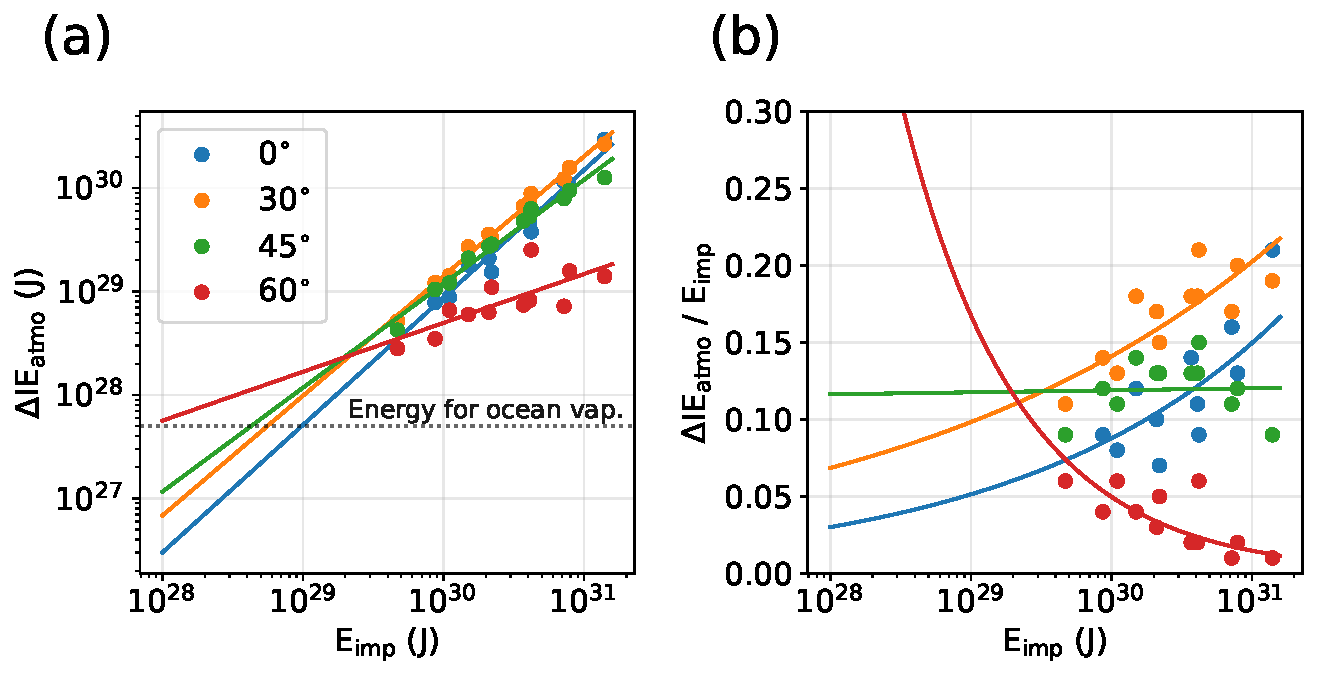
\includegraphics[width=0.8\textwidth]{figures/energy_for_ocean_vap.pdf}
  \caption{\citet{Citron_2022} smoothed-particle hydrodynamics simulations that show how much impactor kinetic energy heats the atmosphere and ocean. Different colors indicated various incident impact angles. (a) shows the simulated change in internal energy of the atmosphere and ocean as a function of the impactor energy, with linear log-log extrapolations for each impact angle. The dotted horizontal line at $5 \times 10^{27}$ J indicates the energy needed to vaporize an ocean \citep{Sleep_1989}. (b) contains the same information as (a), except the y-axis is the fraction of impactor energy that heats the atmosphere and ocean.}
  \label{fig:energy_for_ocean_vap}
\end{figure}

The evaluate the sensitivity of our results to an assumed constant $f_\mathrm{E,vap} = 0.1$, we recomputed the likelihood and timing of a life-starting impact using $f_\mathrm{E,vap} = 0.025$ and $f_\mathrm{E,vap} = 0.25$ (Figure \ref{fig:probabilities_of_impacts_sens} and \ref{fig:timing_sensitivity}). We chose these values because they are reasonable lower and upper bounds based on the \citet{Citron_2022} simulations (Figure \ref{fig:energy_for_ocean_vap}b). The probability of an impact that produces substantial prebiotic molecules without later ocean vaporization decreases with increasing $f_\mathrm{E,vap}$ (Figure \ref{fig:probabilities_of_impacts_sens}). For example, for $f_\mathrm{E,vap} = 0.1$, the probability of a $>4 \times 10^{20}$ kg impact (\citet{Wogan_2023} optimistic case) without subsequent ocean vaporization is 92\%. For $f_\mathrm{E,vap} = 0.025$ and $f_\mathrm{E,vap} = 0.25$ the probabilities are instead 99.9\% and 60\%, respectively.

\begin{figure}
  \centering
  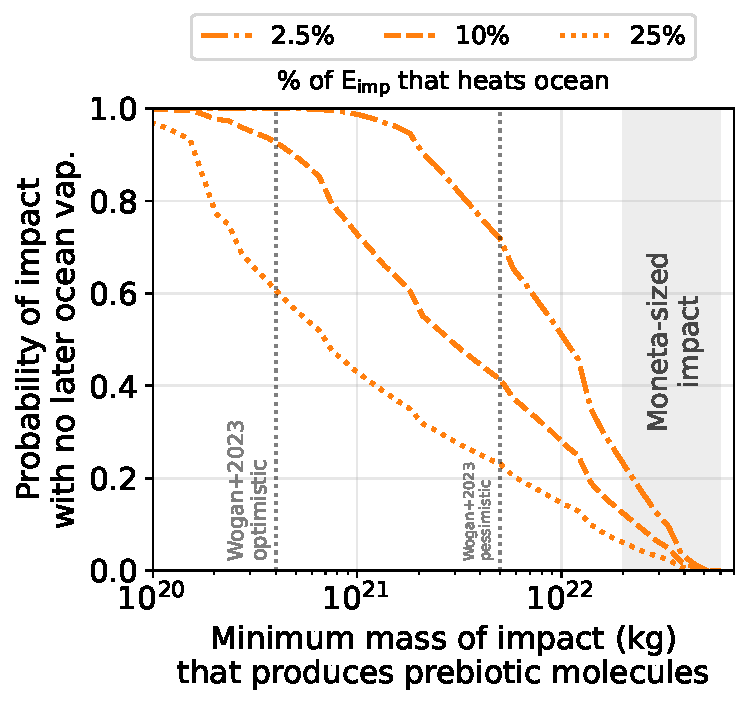
\includegraphics[width=0.5\textwidth]{figures/probabilities_of_impacts_sens.pdf}
  \caption{Similar to Main Text Figure 2, except we consider different values for the fraction of impactor energy that heats the ocean.}
  \label{fig:probabilities_of_impacts_sens}
\end{figure}

Figure \ref{fig:timing_sensitivity} shows the timing of the last impact to make conditions favorable for biopoiesis that does not experience subsequent ocean vaporization for $f_\mathrm{E,vap}$ values of 0.025, 0.1 (nominal value), and 0.25. As in the main text, we consider the \citet{Wogan_2023} optimistic (Figure \ref{fig:timing_sensitivity}a) and pessimistic (Figure \ref{fig:timing_sensitivity}b) minimum impactor masses to produce significant prebiotic molecules. In Figure \ref{fig:timing_sensitivity}a, the timing of the last life-starting impact is relatively insensitive to $f_\mathrm{E,vap}$. In the \citet{Wogan_2023} pessimistic case (Figure \ref{fig:timing_sensitivity}b), an origin of life is preferred later in the Hadean for larger values of $f_\mathrm{E,vap}$.

\begin{figure}
  \centering
  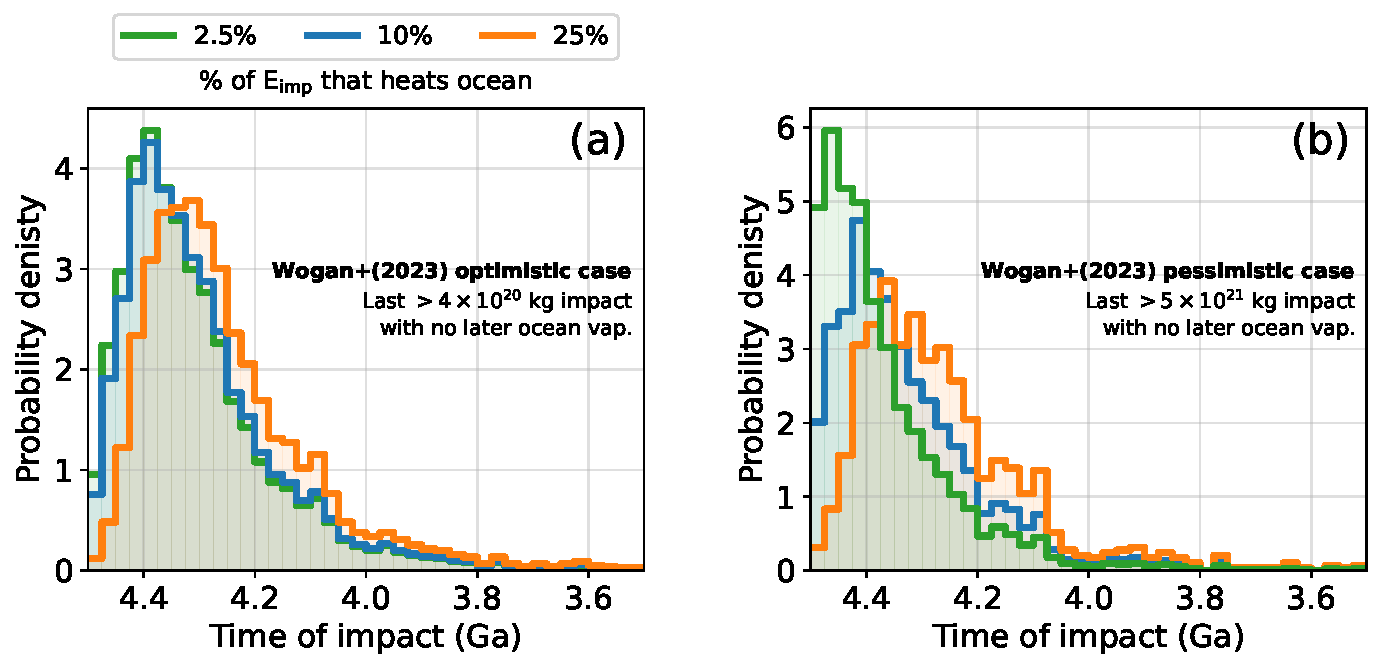
\includegraphics[width=0.85\textwidth]{figures/timing_sensitivity.pdf}
  \caption{Similar to Main Text Figure 3, except we consider different values for the fraction of impactor energy that heats the ocean.}
  \label{fig:timing_sensitivity}
\end{figure}

Overall, uncertainty in the impact properties required to vaporize the ocean has a small effect on our qualitative conclusions. Regardless of $f_\mathrm{E,vap}$, the origin of life on Earth from an impact does not appear to be a fluke (Figure \ref{fig:probabilities_of_impacts_sens}) and biopoiesis is preferred early in the Hadean with uncertainty spanning the entire eon (Figure \ref{fig:timing_sensitivity}). However, it is conceivable that a more complete understanding $f_\mathrm{E,vap}$ as a function of impact angle and other impact parameters could change these results.


\bibliography{bib}
\bibliographystyle{aasjournal}

\end{document}